\def\tutdate{26.01.2017}
\ifdefined\compileall \else
\ifdefined\compiletype
	\documentclass[handout]{beamer}
\else
	\documentclass{beamer}
	\def\compiletype{livebeamer}
\fi

\usepackage{templates/beamerthemekitwide}

\usepackage[utf8]{inputenc}
\usepackage[T1]{fontenc}
\usepackage[ngerman]{babel}
\usepackage{listings}
\usepackage{hyperref}
\usepackage{graphicx}

\usepackage{amsmath}
\usepackage{amsthm}
\usepackage{amssymb}
\usepackage{polynom}

\usepackage{ifthen}
\usepackage{adjustbox} % for \adjincludegraphics

\newcommand{\markBlue}[1]{\textcolor{kit-blue100}{#1}}
\newcommand{\markGreen}[1]{\textcolor{kit-green100}{#1}}

\newcommand{\pitem}{\pause\item}
\newcommand{\p}{\pause}

% -- MATH MACROS
\newcommand{\thistheoremname}{}
\newcommand{\G}{\mathbb{Z}}
\newcommand{\B}{\mathbb{B}}
\newcommand{\R}{\mathbb{R}}
\newcommand{\N}{\mathbb{N}}
\newcommand{\Q}{\mathbb{Q}}
\newcommand{\C}{\mathbb{C}}
\newcommand{\Z}{\mathbb{Z}}
\newcommand{\F}{\mathbb{F}}
\newcommand{\mi}{\mathrm{i}}
\renewcommand{\epsilon}{\varepsilon}


\newenvironment<>{taskblock}[1]{%
	\setbeamercolor{block title}{fg=kit-orange15,bg=kit-orange100}
	\setbeamercolor{block body}{fg=black,bg=kit-orange30}%
	\begin{block}#2{#1}}{\end{block}}

\setbeamertemplate{enumerate items}[default]

% Aussagenlogik Symbole
\newcommand{\W}{w}
\renewcommand{\F}{f}

% Kodierung
\newcommand{\frepr}{\textbf{repr}}
\newcommand{\fRepr}{\textbf{Repr}}
\newcommand{\fZkpl}{\textbf{Zkpl}}
\newcommand{\fbin}{\textbf{bin}}
\newcommand{\fdiv}{\textbf{ div }}
\newcommand{\fmod}{\textbf{ mod }}

\title[Grundbegriffe der Informatik]{Grundbegriffe der Informatik\\Tutorium 33}
\subtitle{}
\author{Lukas Bach, lukas.bach@student.kit.edu}
\date{\tutdate}

\institute{}

\titlelogo{lukasbach}

\titleimage{bg}
%\titleimage{bg-advent}


\ifthenelse{\equal{\compiletype}{livebeamer}}
	{
		\def\livebeamermode{1}
	}{}

\ifthenelse{\equal{\compiletype}{print}}
	{
		\def\printmode{1}
	}{}

\setbeamercovered{invisible}

%\usepackage[citestyle=authoryear,bibstyle=numeric,hyperref,backend=biber]{biblatex}
%\addbibresource{templates/example.bib}
%\bibhang1em

\begin{document}
	
\selectlanguage{ngerman}


%title page
\begin{frame}
	\titlepage
\end{frame}

%table of contents
\ifdefined\printmode
	\ifdefined\compileall \else
	\begin{frame}{Gliederung}
		\tableofcontents
	\end{frame}
\fi\fi

\fi

\section{Komplexitätstheorie}
\begin{frame}{Rückblick}
	\begin{itemize}
		\pitem Was ist $\Omega(f), \Theta(f), \okalk(f)$?
		\pitem Wieso messen wir nicht einfach Laufzeit in ``Anzahl Operationen''?
	\end{itemize}
\end{frame}

\begin{frame}{Obere und untere Schranke}
	\begin{block}{Obere Schranke (Worst-Case Approximation)}
		$O(f) = \{g| \exists c \in \mathbb{R}_+ : \exists n_0 \in \mathbb{N}_0: \forall n \geq n_0 : g(n)\leq c \cdot f(n)\}$
	\end{block}
	
	\pause
	
	\begin{block}{Untere Schranke (Best-Case Approximation)}
		$\Omega(f) = \{g| \exists c \in \mathbb{R}_+ : \exists n_0 \in \mathbb{N}_0: \forall n \geq n_0 : g(n)\geq c \cdot f(n)\}$
	\end{block}

	\pause

	\begin{block}{Average-Case Approximation}
		$\Theta(f) = \{g|\exists c, c' \in \mathbb{R}_+ : \exists n_0 \in \mathbb{N}_0: \forall n \geq n_0 : c \cdot f(n) \leq g(n)\leq c' \cdot f(n)\}$
	\end{block}

	\pause
	
	Auf welche Weise wird hier approximiert? % durch weglassen konstanter faktoren, durch setzen eines n_0, ab dem approximation immer gilt
\end{frame}

\begin{frame}
	Gelten folgende Approximationen?
	
	\begin{itemize}
		\pitem $4n^2 + \pi n + 2 \sqrt{n} \in \Theta(n^2)?$ \pause Ja.
		\pitem $5n^2 + \pi n + 2 \sqrt{n} \in \Theta(n^2)?$ \pause Ja.
		\pitem $4n^{2,1} + \pi n + 2 \sqrt{n} \in \Theta(n^2)?$ \pause Nein.
	\end{itemize}

	\bp Es sind immer nur die höchsten Faktoren interessant!
	
	\begin{itemize}
		\pitem $4n^4 + 3c^6 \in \Theta(n^4)$? \pause Ja\ip, $c$ ist eine Konstante, $3c^6=(3c^6)n^0$ hat eine kleinere Potenz als $n^4$.
		\pitem $\log_{4213}(n) \in \Theta(\log_2(n)$ \pause Ja\ip, die Basis des Logarithmus ist im O-Kalkül egal.
		
		\begin{itemize}
			\pitem Grund: $\okalk(\log_b n) \ip= \okalk(\frac{\log_a n}{\log_a b}) \ip = \okalk(\frac{1}{\log_a b}\log_a n) \ip = \okalk(\log_a n)$.
		\end{itemize}
		
		\pitem $n! \in \Theta(n^{\pi e 2000})$ \pause Nein\ip, Fakultät wächst asymptotisch schneller als fast alles andere.
	\end{itemize}
\end{frame}

\begin{frame}
	Gelten folgende Approximationen?
	
	\begin{itemize}
		\pitem $4n^3 + 2n^2 \in \okalk(n^5)$? \pause Ja.
		\pitem $4n^3 + 2n^2 \in \okalk(n^4)$? \pause Ja.
		\pitem $4n^3 + 2n^2 \in \okalk(n^3)$? \pause Ja.
		\pitem $4n^3 + 2n^2 \in \okalk(n^2)$? \pause Nein.
		\pitem $4n^3 + 2n^2 \in \Omega(n^5)$? \pause Nein.
		\pitem $4n^3 + 2n^2 \in \Omega(n^4)$? \pause Nein.
		\pitem $4n^3 + 2n^2 \in \Omega(n^3)$? \pause Ja.
		\pitem $4n^3 + 2n^2 \in \Omega(n^2)$? \pause Ja.
	\end{itemize}
\end{frame}

\begin{frame}{Aufgabe}
	\begin{taskblock}{Übungsaufgabe}
		Entscheide für jede Zelle, ob die Formel der Zeile in der Menge der Spalte liegt.
		
		\begin{center}
			\begin{tabular}{r||c|c|c|c|c|c}%*{2}{>{$}c<{$}}|*{4}{>{$}c<{$}}
				\hline
				& $\okalk(n^3)$ & $\okalk(n)$ & $\Theta(c!)$ & $\Theta(n^\pi)$ & $\Omega(n^6)$ & $\Omega(n!)$ \\\hline\hline
				
				$2n^2 + 4n$ 
					& \visible<2->{$\in$}
					& \visible<3->{$\not\in$}
					& \visible<4->{$\not\in$}
					& \visible<5->{$\not\in$}
					& \visible<6->{$\not\in$}
					& \visible<7->{$\not\in$}
					\\\hline
					
				
				$\pi$
					& \visible<8->{$\in$}
					& \visible<9->{$\in$}
					& \visible<10->{$\in$}
					& \visible<11->{$\not\in$}
					& \visible<12->{$\not\in$}
					& \visible<13->{$\not\in$}
					\\\hline
				
				$\log(n)$
					& \visible<14->{$\in$}
					& \visible<15->{$\in$}
					& \visible<16->{$\not\in$}
					& \visible<17->{$\not\in$}
					& \visible<18->{$\not\in$}
					& \visible<19->{$\not\in$}
					\\\hline
				
				$n\log(n)$
					& \visible<20->{$\in$}
					& \visible<21->{$\not\in$}
					& \visible<22->{$\not\in$}
					& \visible<23->{$\not\in$}
					& \visible<24->{$\not\in$}
					& \visible<25->{$\not\in$}
					\\\hline
				
				$n^\pi$
					& \visible<26->{$\not\in$}
					& \visible<27->{$\not\in$}
					& \visible<28->{$\not\in$}
					& \visible<29->{$\in$}
					& \visible<30->{$\not\in$}
					& \visible<31->{$\not\in$}
					\\\hline
				
				$12n^3+7000n^2$
					& \visible<32->{$\in$}
					& \visible<33->{$\not\in$}
					& \visible<34->{$\not\in$}
					& \visible<35->{$\not\in$}
					& \visible<36->{$\not\in$}
					& \visible<37->{$\not\in$}
					\\\hline
				
				$n^3$
					& \visible<38->{$\in$}
					& \visible<39->{$\not\in$}
					& \visible<40->{$\not\in$}
					& \visible<41->{$\not\in$}
					& \visible<42->{$\not\in$}
					& \visible<43->{$\not\in$}
					\\\hline
				
				$n!$
					& \visible<44->{$\not\in$}
					& \visible<45->{$\not\in$}
					& \visible<46->{$\not\in$}
					& \visible<47->{$\not\in$}
					& \visible<48->{$\in$}
					& \visible<49->{$\in$}
					\\\hline
				
				%\visible<1->{\F} & \visible<1->{\F} & \visible<5->{\F} & \visible<9->{\F} & \visible<17->{\W} & \visible<13->{\F} \\\hline
				
			\end{tabular}
		\end{center}
	\end{taskblock}
\end{frame}


\begin{frame}
	\begin{itemize}
		\pitem $\okalk (n^2) \cap \okalk(n) = \okalk(?)$? \pause $= \okalk(n)$.
		\pitem $\okalk(n^2) \cap \Omega(n^3) = \pause \emptyset$
	\end{itemize}
\end{frame}

\begin{frame}{Grundlegende Reihenfolge von Größen}
	\begin{center}
		$1 \curlyeqprec \log n \curlyeqprec n \log n \curlyeqprec n^2 \curlyeqprec n^3 \curlyeqprec n^{10000} \curlyeqprec n^2 \curlyeqprec 3^n \curlyeqprec 1000^n \curlyeqprec n! \curlyeqprec n^n$
	\end{center}
\end{frame}

\begin{frame}{Mathematische Definitionen}
	\begin{align*}
	f(n) \in \Omega(g(n)) \Leftrightarrow 0 < \liminf_{n \rightarrow \infty} \frac{f(n)}{g(n)} \leq \infty\\
	f(n) \in \Theta(g(n)) \Leftarrow  0 <  \lim_{n \rightarrow \infty} \frac{f(n)}{g(n)} = c < \infty\\
	f(n) \in \mathcal{O}(g(n)) \Leftrightarrow 0 \leq \limsup_{n \rightarrow \infty} \frac{f(n)}{g(n)} = c < \infty
	\end{align*}
	
	\bp
	
	\begin{taskblock}
		% Aufgaben sind vom ersten Algo Blatt letzten Jahres, Lösung: https://crypto.iti.kit.edu/fileadmin/User/Lectures/Algorithmen_SS16/loesung_01.pdf
		Zeige:
		\begin{itemize}
			\item $3n^2 + 14n + 159 \in \Theta(n^2)$ %a1 a i
			\item $\log n^2 \in \Theta(\log n^3)$ %a1 b ii
			\item $\log^2 n \in \okalk(\log^3 n)$ %a1 b i
		\end{itemize}
	\end{taskblock}
\end{frame}

\begin{frame}{Komplexität mit vollständiger Induktion beweisen}
	% Ebenfalls vom Algo blatt. Vielleicht nur kurz zeigen bzw vorrechnen, eher nur um nochmal vollst Induktion zu zeigen.
	
	\begin{taskblock}
		Zeige mittels vollständiger Induktion:
		\begin{itemize}
			\item $2^n \in \Theta(n^3)$ %a1 a ii
			\item $(n+1)! \in \Theta(n! + 2^n)$ %a1 b iii
		\end{itemize}
	\end{taskblock}
\end{frame}

\begin{frame}
	\begin{tabular}{| r || l |}
		\hline Größenordnung & Bezeichnung\\\hline\hline\ip 
		
		$\okalk(1)$ & konstante Laufzeit \\\hline\ip 
		$\okalk(\log n)$ & logarithmische Laufzeit \\\hline\ip 
		$\okalk(\log^2 n)$ & quadratisch logarithmische Laufzeit \\\hline\ip 
		$\okalk(n)$ & lineare Laufzeit \\\hline\ip 
		$\okalk(n^2)$ & quadratische Laufzeit \\\hline\ip 
		$\okalk(n^3)$ & kubische Laufzeit \\\hline\ip 
		$\okalk(n^k)$ & polynomielle Laufzeit \\\hline
	\end{tabular}
\end{frame}

\begin{frame}
	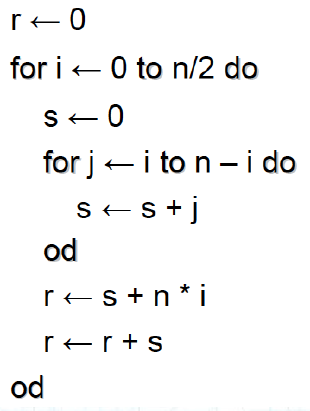
\includegraphics[scale=0.5]{images/okalk_algo.png}
	
	\begin{itemize}
		\pitem Wie oft wird die innere Schleife durchlaufen? \pause $n-2i+1$ mal.
		\pitem Wie kommen wir jetzt auf die Gesamtlaufzeit?
		\pitem $\sum\limits_{i=0}^{n/2} (n-2i+1) \ip = \frac{n}{2}n -2\sum\limits_{i=0}^{n/2}i+\frac{n}{2} \ip = \frac{n^2}{2}+\frac{n}{2}-2\frac{\frac{n}{2}\cdot \left(\frac{n}{2}+1\right)}{2} \ip = \frac{n^2}{2}+\frac{n}{2}-\frac{n^2}{4}-\frac{n}{2}\ip = \frac{1}{4}n^2$
		\pitem Kann man das einfacher machen?
	\end{itemize}
\end{frame}


\subsection{Mastertheorem}

\begin{frame}{Mastertheorem}
	\ip
	\begin{block}{Formel für Mastertheorem}
		\ip Rekursive Komplexitätsformeln der Form\\
		
		\vspace{.2cm}
		\ip$\quad T(n) = a \cdot T(\frac{n}{b}) + f(n)$
		\vspace{.2cm}
		
		\ip lassen sich mit dem Mastertheorem Komplexitätsklassen zuordnen.
	\end{block}

	\begin{block}{Auflösung des Mastertheorem}
		\begin{description}
			\item[Fall 1:] Wenn $f \in \okalk(n^{\log_b a -\epsilon})$ für ein
			$\epsilon>0$ ist, dann ist $T\in \Theta(n^{\log_b a})$.
			\item[Fall 2:] Wenn $f \in \Theta(n^{\log_b a})$ ist, dann ist
			$T\in \Theta(n^{\log_b a}\log n)$.
			\item[Fall 3:] Wenn $f \in \okalk(n^{\log_b a +\epsilon})$ für ein
			$\epsilon>0$ ist, und wenn es eine Konstante $d$ gibt mit $0<d<1$, so
			dass für alle hinreichend großen $n$ gilt $af(n/b)\leq d f$, dann
			ist $T\in \Theta(f)$.
		\end{description}
	\end{block}
\end{frame}

\begin{frame}{Aufgaben zum Mastertheorem}
	\begin{itemize}
		\pitem $T(n) := 2 T(\frac{n}{4}) + \sqrt{n}$\pause, also $a=2, b=4, f(n) = \sqrt{n}$\pause, also zweiter Fall des Mastertheorems\pause. $T \in \Theta (\sqrt{n}\log n)$
		\pitem $T(n) := 3 T(\frac{n}{2}) + n\log n$\pause, also $a = 3, b=2, f(n) = n\log n$\pause, also erster Fall des Mastertheorems\pause, $T \in \Theta(n^{\log_2 3})$
		\pitem $T(n) := 4 T(\frac{n}{2}) + n^2\sqrt{n}$\pause, also $a = 4, b=2, f(n) = n^2\sqrt{n}$\pause, also dritter Fall des Mastertheorems\pause, $T \in \Theta(n^2\sqrt{n})$.
	\end{itemize}
\end{frame}

%\subsection{Beweisaufgaben}

%\begin{frame}{Beweisaufgabe zu O-Kalkül}
%	\begin{taskblock}{Beweisaufgabe}
%		Zeige, dass gilt: $3n^3 \not\in \okalk(n^2)$.
%	\end{taskblock}
%
%	\pause
%	
%	Annahme: \ip $3n^3 \in \okalk(n^2)$. 
%	
%	\ip Dann gilt: $\exists c \in \R_+ : \exists n_0 \in \N_0 : \forall n \geq n_0 : \ip c\cdot 3n^3 \leq n^2$.
%	
%	\ip Da der linke Term möglichst klein sein soll\ip, können wir $c < 1$ setzen. \ip Sei $k_0 = \%lceil c \rceil ^{-1} \geq c^{-1}$.
%	
%	\ip Dann: $c \cdot 4k_0^3 = c \cdot k_0 \cdot 3k_0^2 \ip = 3m \cdot k_0^2 \ip \geq k_0^2$ \ip ($m$ durch den Rundungsrest).
%	
%	\ip $m > 1$ und $\forall k \in \N_0, k \geq k_0 : 3k^3 > k^2$.
%\end{frame}


\section{Automaten}

\begin{frame}{Definition eines endlichen Automaten}
	\begin{block}{Endlicher Automat}
		Ein endlicher Automat ist ein Tupel $A = (Z, z_0, X, f, Y, g)$ mit...
		
		\begin{itemize}
			\pitem endliche Zustandsmenge $Z$
			\pitem Anfangszustand $z_0 \in Z$
			\pitem Eingabealphabet $X$
			\pitem Zustandsübergangsfunktion $f: Z \times X \rightarrow Z$
			\pitem Ausgabealphabet $Y$
			\pitem Ausgabefunktion 
			\begin{itemize}
				\pitem Mealy-Automat: $g: Z \times X \rightarrow Y^*$
				\pitem Moore-Automat: $h: Z \rightarrow Y^*$
			\end{itemize}
		\end{itemize}
	\end{block}
\end{frame}

\ifdefined\compileall
\else


\ifthenelse{\equal{\compiletype}{print}}
{

\begin{frame}{Informationen}
	
	\begin{columns}
		\begin{column}{0.5\textwidth}
			
			\begin{block}{Zum Tutorium}
				\begin{itemize}
					\item Lukas Bach
					\item Tutorienfolien auf: 
					\begin{itemize}
						\item \url{http://gbi.lukasbach.com}
					\end{itemize}
					\item Tutorium findet statt:
					\begin{itemize}
						\item Donnerstags, 14:00 - 15:30
						\item 50.34 Informatikbau, -107
					\end{itemize}
				\end{itemize}
			\end{block}
			
			\begin{block}{Mehr Material}
				\begin{itemize}
					\item Ehemalige GBI Webseite:
					\begin{itemize}
						\item \url{http://gbi.ira.uka.de}
						\item Altklausuren!
					\end{itemize}
				\end{itemize}
			\end{block}
			
		\end{column}
		\begin{column}{0.5\textwidth}
			
			\begin{block}{Zur Veranstaltung}
				\begin{itemize}
					\item Grundbegriffe der Informatik
					\item Klausurtermin:
					\begin{itemize}
						\item 06.03.2017, 11:00
						\item Zwei Stunden Bearbeitungszeit
						\item 6 ECTS für Informatiker und Informationswirte, 4 ECTS für Mathematiker und Physiker
					\end{itemize}
				\end{itemize}
			\end{block}
			
			\begin{block}{Zum Übungsschein}
				\begin{itemize}
					\item Übungsblatt jede Woche
					\item Ab 50\% insgesamt hat man den Übungsschein
					\item Keine Voraussetzung für die Klausur, aber für das Modul
				\end{itemize}
			\end{block}
			
		\end{column}
	\end{columns}
	
\end{frame}

}{}

\ifdefined\livebeamermode
	\begin{frame}
		
\includegraphics[width=\linewidth]{images/thatsall.png}
	\end{frame}
\fi

\end{document}

\fi